
% Added link to preamble
\documentclass[english,12pt]{article}
\usepackage{hyperref}
\usepackage[utf8]{inputenc}
\usepackage{blindtext}
\usepackage{graphicx}
\usepackage{authblk}
%\usepackage{natbib}
\usepackage{xcolor}
\usepackage{float}
\usepackage{amsmath}
\usepackage[english]{babel}
\usepackage{graphicx} % Required for inserting images
\usepackage[paperheight=16cm,paperwidth=12cm,textwidth=8cm]{geometry}
\usepackage[flushleft]{threeparttable,booktabs}
\usepackage{tabulary,booktabs}
\usepackage{booktabs}
\usepackage{siunitx}
\usepackage{ragged2e}

\appto\TPTnoteSettings{\footnotesize}

\usepackage[
        backend=biber,
        style=authoryear-comp,
        sorting=nyt,
        style=apa
    ]{biblatex}
 \addbibresource{references.bib}


 \geometry{
 a4paper,
 total={170mm,257mm},
 left=30mm,
 right=30mm,
 top=30mm,
 bottom=30mm
 }

% Keywords command
\providecommand{\keywords}[1]
{
  \small	
  \textbf{\textit{Keywords---}} #1
}

\graphicspath{{output/}}


\addbibresource{}

% Here the packages used, please do not remove
\usepackage{xcolor}



\title{Trust and diversity as an outcome of associative behavior patterns}
\author{Roberto Cantillan$^{1}$, Gustavo Ahumada$^{2}$, Vicente Espinoza $^{3}$  \\
        \small $^{12}$Pontificia Universidad Católica de Chile \\
        \small $^{3}$Centre for Social Conflict and Cohesion Studies COES \\
}

\date{Junio 2023}


\begin{document}
\maketitle


\begin{abstract}
En línea con la tradición analítica de redes, buscamos profundizar en la conexión entre el comportamiento asociativo (o cívico asociativo) y resultados de capital social a nivel individual. De esta manera, nos enfocamos en las "membresías múltiples", entendidas como un mecanismo básico de constitución de un campo de relaciones interorganizacionales, y la emergencia de patrones estratificados en términos de composición y de alcance asociativo. Adicioanlmente, buscamos profundizar en la hipótesis de Putnam, la cual sugiere que las membresías asociativas se asocian positivamente con la confianza generalizada, sugiriendo que son los patrones más diversos de membresías (en efecto, aquellos que facilitan el acceso a círculos y posiciones sociales diversas) los cuales facilitan en desarrollo de capital social a nivel individual y colectivo (confianza generalizada, confianza vecinal y diversidad de contactos ocupacionales)
\end{abstract}
\hspace{10pt}

\keywords{Multiple memberships, Social capital, Trust, associative field} 

\newpage


\maketitle

\section{Introduction}

That people and communities can benefit from membership in voluntary associations is by no means a novel idea. Literature in this field has established that voluntary associations promote and enhance social relations with non-kin as well as generalized trust. Involvement in association’s activities operate as a school of civicness where individuals learn to manage their differences and process their conflicts by extending their knowledge and tolerance to people from other social circles. In addition, some researchers argue that the activation of personal ties in associations, although initially based on similar interests can help to reach distant social circles, favoring the access to scarce social resources.
\bigskip
 
To what extent positive outcomes associated accompanying voluntary associations hold in contexts of noticeable material inequality and social exclusion? In this paper we analyze the Chilean case to discuss the extent to which membership in voluntary associations contributes to social trust as well as a bridge to distant social circles. We argue that positive effects of associations regarding generalized and local trust can be discerned even in an unfavorable context. However, the quality of their connections with other voluntary organizations has a stronger effect than the type of organization.
\bigskip

Neoliberalism in Latinamerica goes hand in hand with increasing levels of social and political inequality, supported by a substantial concentration of economic resources \parencite{sassen_expulsiones_2015}. Social structure in most Latin-American countries consists of a small self-reproducing elite, a group of people below the income poverty line and roughly 70  percent of the population who is neither poor or rich. Indeed, a large proportion of the latter make do in a context of increasing uncertainty and insecurity, often engaged in informal employment \parencite{lomnitz_lo_2008, portes_free-market_2005, schneider_economic_2008}. In spite of a decreasing income poverty most of the population is vulnerable to a relapse into poverty as a consequence of individual setbacks as well as external shocks. Social policies since the 1990s in spite of their contribution to decrease acute poverty, did not revert high material inequality or offered sustainable gains to the population.
\bigskip

Neoliberal orientations somehow got ingrained in the dynamics of Chilean society fueling its long term operation. During the 1970s and 1980s, the Chilean dictatorship systematically destroyed the solidarity links in society, by sheer repression of organizations such as unions, neighbors' groups, students associations and the like. The dictatorship also dismantled the institutional support for solidarity by privatizing public services, especially pensions, education and health. On top of political repression and privatization of public services an ideology of individual achievement undermined the social fabric of Chilean society. Moreover social life itself was retracted to the private world, comprising kin and a small number of friends and acquaintances in highly homogeneous social circles (REF). Disconnection among people decreased trust in strangers hindering the conditions for collective action (Lechner ). 
\bigskip

Voluntary associations, however, continued to exist, especially in local contexts, although they are small in size and operate without coordination \parencite{espinoza_local_2013}. Voluntary associations in Chile do not match exactly the characteristics they have in the United States or Europe. Chilean groups operate at a small scale, usually associated with a neighborhood; some intend to represent the inhabitants before local authorities and others gather people with common interests (for instance, housing, recreation, sports, etc.). They usually obtain financial resources from several government funds intended to support social organization \parencite{alenda__2013}. This mechanism of public funding has affected the quality of associations because it stimulated the competition for resources among associations. Leaders of the organizations learned to compete with each other rather than cooperate, which affected the civic attributes of voluntary associations. It is debatable to what extent they meet the qualities usually associated with social capital \parencite{delamaza_sociedad_2002, espinoza_local_2013}. 
\bigskip

On top of an exclusionary model of development, individualization of social life and weak voluntary associations, political institutions have clear shortcomings in processing social and political demands, contributing to the accumulation of social discomfort. As a matter of fact the Chilean “social outburst” of October 2019, actually heralded a cycle of protest that lasted until March 2020 and was only interrupted by the sanitary crisis associated with COVID-19. Chilean protest gave way to multifarious demands pointing to a deep change in the political and economic system. We conjecture to what extent protests can be linked to many types of voluntary associations, that sheltered the many pursuits expressed in these demonstrations. (REF)
 \bigskip
 
In this paper we wonder to what extent membership in Chilean voluntary associations promotes or hinders social trust among its members. The interest of the paper has to do with the test of well-established hypotheses about the benefits of voluntary associations in a different cultural, social and political context. In the first part we contextualize and develop the theoretical argument that supports our hypotheses. We then proceed to analyze our data focusing on two levels: 1) First, we focus on the search for emerging patterns of connectivity that shape the structure of the associative field in Chile, and 2) we evaluate the effects of individual memberships in two ways of social capital: trust (local and generalized) and diversity of personal networks. Finally, we discuss our results and conclude


\subsection{Civil society in Chile and Latin America in the neoliberal phase}

The passage of time revealed the profound transformations in the relationship of the popular sectors with politics, which began with the neoliberal reforms. The neoliberal context is characterized by the replacement of the state-centric forms of the state-citizenship relationship, based on corporatism and the dominant developmentalism in Latin America until the 1970s \parencite{oxhorn_neopluralism_2004}. Instead, a market-centric pattern of state-citizenship relationship was deployed. This pattern was characterized by deploying targeted forms of incorporation and distribution of incentives, with the objective of integrating the “poor” into the market. 
\bigskip

In organizational terms, if the national popular period was characterized by the selective incorporation of popular actors in the political sphere (for example, trade unions), neoliberal reforms were the expression of the efforts of political and economic elites to exclude and weaken popular actors and their organizations, restricting their ability to influence the formulation of socioeconomic policies \parencite{collier_shaping_1991, cook_politics_2009, espinoza_local_2013, rossi_second_2015, silva_reshaping_2018}. 
\bigskip

In this scenario the traditional collective actors of the popular national matrix: unions and parties, lost their centrality \parencite{barozet_entre_2016,espinoza_local_2013,garreton_cambios_2001} and, with it, their role as intermediaries between the classes popular and the State. For the Chilean case, Espinoza (2013) suggests that the effects of neoliberal policy oriented towards the development of contests and competition for access to resources by vulnerable groups, establishes exchange relationships based on conflict instead of cooperation, which fragments local spaces and reduces solidarity between diverse groups. 
\bigskip

At the Latin American level, new popular actors with a territorial base emerged, such as indigenous peoples movements, unemployed workers, residents of marginal neighborhoods, homeless, and landless peasants \parencite{merklen_pobres_2010, rossi_second_2015, seoane_nuevas_2006, svampa_movimientos_2010}. In this context, the trade union movement was one more participant among many in the anti-neoliberal protests, and its relationship with the territorial movements varied greatly from case to case \parencite{silva_challenging_2009}. 
\bigskip

Although a heterogeneous and polycentric structure of organizations may indicate a field rich in experiences of collective action (United Nations Development Programme, 2000), integration and the capacity to mobilize resources is not assured and depends on social groups that act as bridges between these multiple experiences of collective action \parencite{baldassarri_integrative_2007, granovetter_strength_1973}. One of the characteristics that make up Chilean civil society in particular is the low capacity of popular organizations to fill structural holes. In this way, the identity heterogeneity of civil society is not accompanied by weak links between organizations, so it is plausible that the capacity for interaction, the flow of resources and solidarity is restricted. This pattern is particularly critical since the absence of stable links of cooperation and / or conflict between entities that make up a social space can also be described as a context with high levels of polarization \parencite{aref_detecting_2020}.
\bigskip

On the other hand, popular influence on public policy is less likely when channels are strongly individualized. Along these lines, the academics argued that unlike unions and other corporatist groups, the new organizations lacked party ties or privileged access to policy makers, limiting their ability to represent popular interests \parencite{collier_reorganizing_2009, silva_reshaping_2018}.
\bigskip

As the state withdrew from its basic functions, it put out to tender the space of social services. Popular demand was assumed by new non-governmental organizations (NGOs) that filled the void by providing critical services to the population  \parencite{boulding_community_2020, holzner_poverty_2007}. Many of these organizations (the vast majority of them non-profit) constituted a market that regulates the system of individual and organizational interdependencies in a focused manner, while efficiently distributing public resources to vulnerable populations. The great problem with this type of organization is that its activity is not aimed at building and / or strengthening popular coordination networks that can be constituted as links of democratic participation and governance. On the contrary, its main interest is to meet the particular and critical demands of vulnerable populations (for example, care for vulnerable minors, assistance to individuals with drug use problems, construction and basic housing), establishing dependency relationships with individuals and family nuclei. Put this way, the coordination created by this type of organization tends to be focused on individuals and to depend on permanent state surveillance \parencite{delamaza_redes_2012}.
\bigskip


\section{Theory}

Confidence in others (unknown) is one of the lowest compared to other countries in the region (Latinobarómetro). The "infrasocialized" explanations point to individuation processes marked by the ideology of individualistic entrepreneurship \parencite{araujo_desafios_2012, yopo_individualizacion_2013}. The "over-socialized" explanations point to the pressure of a system of norms that leaves little room for collective action and the development of public interest \parencite{oxhorn_neopluralism_2004}. Low civic rates and general collective participation \parencite{espinoza_capital_2009}.

- ciucuito de conectividad que desarrollan los individuos 


Chile has the lowest level of confidence in others (unknown) in the region (Latinobarómetro). This finding could be understand 

Infrasocialized explanations point to process of individualization characterized byan individualist entrepreneur'sideology

\subsection{The structural bases}

The importance of memberships and patterns of interaction between voluntary associations is by no means a new idea \parencite{diani_cement_2015, sorenson_when_2014}. However, even though much of the research is based on an underlying relational theory, much of the analytical work uses aggregative descriptions to identify patterns of composition of civil society \parencite{salamon_social_1998} or ideational indicators of "cohesion" to describe the benefits of memberships \parencite{paxton_social_2002, paxton_association_2007,putnam_making_1994}. Political sociologists focus on how a cohesive civil society promotes democracy \parencite{paxton_is_1999, putnam_bowling_2000}.  Historical sociologists point to the importance of solidarity for revolutionary action \parencite{bearman_structure_1993, gould_multiple_1991}. Social epidemiologists argue that a cohesive "core" is responsible for the persistence of sexually transmitted diseases \parencite{rothenberg_personal_1996}. \textbf{We need to close the idea of this paragraph. What is the main purpose in this paragraph?}


\bigskip

{\color{blue} The significance of memberships and patterns of interaction among voluntary associations has long been recognized \parencite{diani_cement_2015, sorenson_when_2014}. However, despite the research being grounded in an underlying relational theory, much of the analytical work relies on aggregated descriptions to identify the composition of civil society \parencite{salamon_social_1998} or utilizes ideational indicators of "cohesion" to delineate the benefits of memberships \parencite{paxton_social_2002, paxton_association_2007,putnam_making_1994}. Political sociologists examine how a cohesive civil society fosters democracy \parencite{paxton_is_1999, putnam_bowling_2000}, while historical sociologists emphasize the importance of solidarity for revolutionary action \parencite{bearman_structure_1993, gould_multiple_1991}.}


\bigskip

Structural-relational explanations point to fragmentary interaction patterns and are restricted to primary circles \parencite{castells_globalizacion_2005}. Strong polarization in the associative field and state-citizenship interaction mediated by individuals or interest groups. Collective action unfolds in highly competitive territorial contexts. Vertical fragmentation between popular and state politics (polycentric field). Low membership rate. Precarious state financing \parencite{alenda__2013}. Here, we have five sentences, but they are not related. How are the structural-relational explanations and collective actions linked? May be this question could guide the paragraph. {\color{blue}Here, we have five sentences, but they are not related. How are the structural-relational explanations and collective actions linked? May be this question could guide the paragraph.}

\subsection{Associative field, Quantity versus relations}

Voluntary associations are foci of social activity other than family, work and educational spaces \parencite{knoke_associations_1986}. In this sense, memberships have been understood as a structural characteristic that can increase the probability of acquaintances formation \parencite{mcpherson_hypernetwork_1982} and, at the aggregated level, contribute to the formation of patterns of intergroup interaction and differentiation \parencite{blau_exchange_1986}. For this reason, its ability to affect social capital distribution patterns in populations has been highlighted by the literature \parencite{benton_uniters_2016,diani_social_1997,feld_focused_1981,glanville_voluntary_2004,son_social_2008,tindall_network_2012}.
\bigskip

Voluntary associations are both institutions and networks embedded in broad contexts. Its deployment facilitates the emergence of an infrastructure of exchanges and interdependencies that constitute the “interstitial” field of civil society \parencite{crossley_networks_2018,diani_cement_2015,lee_when_2016}. The configuration of the field of civil society consists of a particular pattern of links (present and absent) between the set of organizational dyads \parencite{kenis_how_2002}. These patterns determine the distribution of restrictions and opportunities that affect the results of the action of the organizations and of the members of the organizations \parencite{paxton_association_2007,son_social_2008,tindall_network_2012} 
\bigskip

Along these lines, it has been suggested that memberships (conceptualized as an expression of civic commitment) contribute to improving accessibility and / or counteracting deficits in individual and collective social capital \parencite{benton_uniters_2016,small_villa_2004,son_social_2008}. On the other hand, its role as a mechanism for the integration of societies and functioning of democratic institutions has been recognized. For example, when the effect on the production of individual cognitive dispositions of tolerance and / or trust in other strangers is indicated {\color{blue} (indicated about what?)}  \parencite{cote_social_2015,putnam_bowling_2000,tocqueville_democracy_1980}. Put like this, the benefits of memberships can be individual or collective, while contributing to the development of social capital in terms of form and content {\color{blue} (this sentence does not make sense, close the idea)}  \parencite{moody_building_2009}. 
\bigskip

Voluntary associations provide an organized context for joint activities, so participation in organizations is likely to shape social networks {\color{blue} (in what sense is similar to social network. Is it provided an organized context?)} \parencite{feld_focused_1981,mcpherson_social_1992}. In general, the analysis of social networks and associations emphasizes two aspects 1) Networks and associations are treated as contexts for socialization and the development of social cohesion. This perspective tends to emphasize mechanisms that facilitate the regulation and establishment of norms, identities, and generalized trust \parencite{glanville_voluntary_2004,glanville_why_2016,paxton_association_2007,paxton_trust_2018} - public good Networks and associations are considered sources of inequality, before which individuals develop strategies to access resources and positions of influence \parencite{bekkers_social_2008} - privileged-good view. The latter is the perspective adopted by this article.

\bigskip

The logic is that greater associative contact in instances of organizational solidarity not only generates greater affection and civic virtues in general, but also has a diversifying effect on the social networks of the actors and, therefore, increases the probability of access to scarce resources \parencite{diani_social_1997,malinick_network_2013,tindall_network_2012,benton_uniters_2016}. In simple terms, it is plausible that participation in social movements fosters the development of social capital at the individual level, that is, in those who declare to be members or participate in social movements. 
\bigskip

Even though some have developed optimistic diagnoses about the development of civil society and the civic activity of popular groups in Latin America and Chile, especially after what some authors call "second incorporation" or " post-neoliberal reincorporation” \parencite{rossi_second_2015}, many of these analyzes have focused on the aggregate count of organizational experiences. For the Chilean case, \parencite{programa_de_las_naciones_unidas_para_el_desarrollo_desarrollo_2000} and the working group led by  Irarrazaval & Streeter \citeyear{irarrazaval_chile_2017}, reported an unexpectedly rich and apparently dense reality of experiences of autonomous collective action organization. However, the perspective and, in some cases, the data used in these studies do not allow testing hypotheses associated with the structure of exchanges between types of voluntary associations or organizations. For the argument we developed, inferring a relationship structure is particularly critical. A structural approach should bring us closer to meeting that goal. We assume that any positive effect that associative life has on individuals and groups, depends on scenarios of fragmentation and segregation in the field of individual and group relationships in which the subjects are embedded. Regarding this, our aim is to analyze the emerging structure of interconnection between associative types observing the multiple memberships of individuals. According to Moody and White  \citeyear{moody_structural_2003}, this analytical focus links two levels of action: individual and organizational, and allows direct analysis of the link between local interaction and patterns of organizational intersection. The logic is that if a member belongs to two or more associations, it links those associations and thus creates a network between the associations \parencite{moody_structural_2003}. Indeed, the more independent pathways there are between groups, the more easily ideas and attitudes flow through them \parencite{moody_structural_2003}.
\bigskip

Interaction patterns between associations and not the mere number of experiences largely determine the integration of the civil society field, and the probability of exposure to diverse people (in relation to the perspective of Lester M. Salamon). The expansion of the personal networks of the members to more than one organization also creates networks between voluntary associations \parencite{moody_structural_2003, kenis_how_2002}, which may allow the transfer of resources and the trust developed within organizations towards others more or less similar. The extension of trust to distant circles involves making an assessment of the trustworthiness of individuals who do not know each other directly, which suggests that the parties are likely to focus on the predictability of each other's behavior or the average person \parencite{glanville_why_2016, paxton_association_2007, paxton_is_2015}
\bigskip

They are constituted as informal networks that depend on multiple memberships and the informal contact of members of diverse organizations. There are associations that probably overlap more with others as a result of the number of relationships that their members have with members of other associations. A proxy identified by the literature is multiple memberships \parencite{moody_structural_2003, paxton_association_2007,pena_lopez_capital_2018}. 
\bigskip

Associative field: Is made up of 1) Patterns of individual civic behavior, 2) Interaction patterns between associations and composition. 

\subsection{The duality of individual behavior and the associative structure
How to analyze multiple memberships?}

As we indicated previously, the associative field is constituted through the interdependence of individual and group identities. This duality refers to the complementarity of relationships between actors as participants in events and between events as collections of actors. That is, personal identities are formed through membership in multiple and differentiated types of groups, and individuals, through their memberships in different types of social groups, provide connections between associations that help shape collective identities ( P. Bonacich, 1972, Breiger, 1974, Diani, 2015, Wasserman & Faust, 2013). In this way, by forming networks embedded in particular contexts but which most likely intersect with each other, control and the achievement of individual and collective objectives are facilitated, while at the same time, a structural order with its qualities emerges (Kontopoulos, 1993; Mann, 1991; White, 2008). Network analysts have traditionally used affiliation matrices to analyze this type of emerging process, however other approaches are referenced in the following table:
\bigskip

In general, the multiple memberships of individuals are a fundamental topic in political and organizational sociology. As some authors indicate \parencite{friedkin_social_2004,moody_structural_2003}, this proxy allows us to understand the processes through which cohesive groups intersect and social integration processes can be developed on larger scales \parencite{blau_inequality_1977}. Table \ref{table: table1} shows that research has used different but similarly sophisticated techniques and measures to address multiple memberships. A significant difference is the focus on variables or individual behavior. On the one hand, we bet that an analysis that uses affiliation matrices to analyze unique associative behavior patterns (from a Bayesian perspective) and, on the other, interdependent group properties improve visualization and understanding of conformation processes. of the associative field.
\bigskip

When the focus is on the variables, that is, on the associations, information is produced about their attributes and the ability of the groups to develop connectivity with their environment and influence the perceptions and attitudes of the members. The latter emphasizes the constriction capacity of particular associations that are more or less connected (understood as contexts). In this way, this approach can be understood as one that pays attention to organizational social capital. For its part, the course from the latent variables focuses on producing emergent profiles of associative behavior from the analysis of the response patterns of individuals. The profile yields information on the probable conduct of individuals based on belonging to population classes. Eventually, it makes it possible to identify those profiles that facilitate access to various organizational contexts, such as those that do so redundantly. The latter allows us to understand how probable behaviors group associations into blocks, at the same time that they can contribute to the formation of attitudes in members. Put like this, this way of approaching multiple memberships can be defined as a proxy of the individuals' social (civic) capital.
\bigskip

\begin{table}[H]
\footnotesize 
\label{table: table1}
\setlength{\tymin}{40pt} % not so narrow columns
% use \RaggedRight instead of \raggedright
\let\raggedright\RaggedRight

\begin{tabulary}{\textwidth}{@{}LLLL@{}}
\toprule
\textbf{Tecnique} &
  \textbf{Papers} &
  \textbf{Foci} &
  \textbf{Measure} \\
\midrule
Summation    & Putnam (2000) Cigler (2002) Erickson (2009; 2004) Glanville (2004; 2016) Magee (2008) Tindal y Cormier (2008) Bekkers et al. (2008) 
             & Extensión de membresías individuales
             & Diversidad de las membresías individuales\\

Overlapping  & Bonacich (1972) (Breiger, 1974) Mizruchi y Galaskiewicz (1994) Mizruchi et al. (1992) Borgatti (2009) Cornwell y Harrison (2004) Diani (2009; 2015) Uzzi (1997) (McPherson, 1982) 
             & Actor/group duality. Detection of clusters and centrality of collective entities
             & Influence and power of entities (similarity, centralization, and centralities)\\
Standardized descriptive  & Paxton (2007) Alenda (2013) 
                          & Organizations, according to their ability to concentrate on bridging opportunities
                          & (Extension of) organizational connectivity\\
Latent variables  & Pena-Lopéz (2018)  
                  & Organizations, according to their ability to concentrate on bridging opportunities
                  & Individual behavior profiles\\
\bottomrule
\end{tabulary}

\caption{Approaches to the study of multiple memberships}
\label{}

\end{table}

\bigskip



\subsection{Associativity and generalized trust}

Trust is an emerging social phenomenon \parencite{kuwabara_cohesion_2011,tilly_confianza_2010}. In psychological terms, it can be defined as a set of socially learned expectations \parencite{barber_logic_1983} that can be deployed between individuals, social circles, and projected towards institutions of various kinds. Trust thus includes the probability of the emergence of a willingness - conscious or unconscious - to trust other "strangers" or strangers, situated in social circles with which there is no direct connection or reciprocal relationships.
\bigskip

The extension of trust to distant circles involves making an assessment of the trustworthiness of individuals who do not know each other directly (the other generalized “strangers”), which suggests that the parties are likely to focus on the predictability of each other's behavior or the average person \parencite{glanville_why_2016,paxton_association_2007,paxton_is_2015}. The logic of the argument is as follows: if the person is known, trust is determined by previous experiences. This could be called private or knowledge-based trust \parencite{yamagishi_trust_1994,stolle_clubs_2001}. Second, if the person is not known, generalization from experience with others is used \parencite{hardin_conceptions_2001}. In this sense, generalized or depersonalized trust is the perception that the generality of society is trustworthy \parencite{glanville_social_2013,paxton_social_2002,paxton_association_2007}. However, this generality can be more or less abstract, which is why its evaluation requires considering levels of trust extension, for example, levels of trust in neighbors or people in the neighborhood, in conjunction with higher levels \parencite{glanville_why_2016}.
\bigskip

In general, associative activity is expected to generate pro-social attitudes in the members for two reasons: 1) In the associative activity, norms of cooperation are experienced, thus arising perceptions of mutual trust among its members. 2) And, because, routine meetings ensure that a potential confidant participates in repeated interactions with the other members of the group, allowing future sanctions against any broken trust \parencite{axelrod_evolution_1984,paxton_trust_2018}. The power of these mechanisms is based on their ability to increase the predictability of interactions, to the extent that people update their expectations of trusted interactions based on whether previous expectations were met \parencite{paxton_trust_2018}. However, Paxton \citeyear{paxton_association_2007} suggests that what is at stake in understanding the creation of generalized trust depends to a large extent on mechanisms that facilitate the extrapolation of the trust produced within the identity limits of the groups towards the other strangers. 
\bigskip

The overlapping of organizations facilitates the creation of acquaintances between distant circles that do not interact frequently, which can motivate the moral ties of the organizational “we” to be expanded through the multiple affiliations of its members, a question that should be empirically investigated for the different cultural and institutional contexts. For this, it is suggested as relevant to analyze two fundamental mechanisms: 1) the extension of diversity, through which the content of the networks is analyzed, that is, the composition of the associations and, 2) the extension of connectivity to through which the form and scope of links between organizations in the fields is analyzed \parencite{paxton_trust_2018}. Along these lines, we suggest two hypotheses:
\bigskip


\subsection{Voluntary associations and diversity}

An extensive body of research has focused on the role of social media in recruiting and activating memberships in voluntary associations and in the deployment of particular collective action coordination modes, such as social movements \parencite{gould_collective_1993,mcpherson_social_1992,tilly_mobilization_1978}. However, there has been less emphasis on the role of memberships in the form of personal social networks \parencite{benton_uniters_2016,tindall_network_2012}.
\bigskip

As we indicated above, it is feasible to expect that the associations most connected with their organizational environment will be foci of social activity that facilitate the intersection of diverse people and social circles, which, in turn, increases the probability of the formation of acquaintances by its members. These “known” potentials may be similar in some respects (for example, in the interest of participating in a particular type of association) but probably dissimilar in many others \parencite{erickson_social_2003}. In this way, through memberships individuals can disrupt (or reaffirm) the content and form of their personal networks. For example, increasing the range of occupations and resources achieved through the links formed in these settings, even when they are weak \parencite{benton_uniters_2016,magee_civic_2008,son_social_2008}. Given this, we suggest the following hypotheses:

\subsection{Hypothesis} 

\begin{itemize}
  \item H1: The associative behavior pattern that most connects to other associative types is positively related to generalized trust and the diversity of personal networks. 
  \item H2: The most closed associative behavior patterns (closure) are negatively related to generalized trust and the diversity of personal networks 
\end{itemize}





\section{Methodology}

In general, the analyzes of the associative field in Chile have been carried out transversally and with a markedly institutional perspective \parencite{irarrazaval_chile_2017,irarrazaval_sociedad_2017, programa_de_las_naciones_unidas_para_el_desarrollo_desarrollo_2000}. In this context, our bet is to analyze the individual/group duality \parencite{breiger_duality_1974, mcpherson_hypernetwork_1982}, taking advantage of the longitudinal data available for the Chilean case. Specifically, we focus on individual-reported associative memberships and emerging patterns of associative interaction. The analysis is carried out in two stages: First, the subjects are classified using an unsupervised learning analytic technique \parencite{molina_machine_2019} according to their response patterns in the three study waves. We model the putative heterogeneity of associational behaviors at the national level using the latent (or hidden) Markov model technique \parencite{bartolucci_latent_2015}, which is specially designed to analyze continuous longitudinal and categorical data. In a second moment, we seek to explain the general confidence considering the individual classification for the three times as an independent variable.  At this stage, we use identification techniques to discover heterogeneous causal effects of associative interaction patterns.
\bigskip



The procedures have been performed with the LMest package \parencite{bartolucci_lmest_2020} designed for R environment. 

\section{Data and variables}
The primary source of data used in this research is the \textit{Estudio Longitudinal de Chile} (Longitudinal Social Study of Chile) (ELSOC). ELSOC is a unity national population-representative panel survey, which annually interviews a sample of Chilean adults (18 or older) in urban areas (cities with more than 10,000 inhabitants) since 2016.\footnote{Additional methodological details about the survey is available at the Data Repository of the Center for Social Conflict and Cohesion Studies (COES) in the Harvard Dataverse \url{https://dataverse.harvard.edu/dataverse/coes_data_repository}}. The last wave was applied at the end of 2022 after the Coronavirus pandemic restrictions. In our analysis, we will use up three out six waves of ELSOC, the reason is that the variables of membership in voluntary organizations were measured in wave 1, 3, and 6. Our analytical sample is restricted to individuals with three observations, which guarantees a balanced panel. 

\bigskip

Our main dependent variable is social trust (\textit{"Generally speaking, would you say that most people can be trusted, or that you have to be careful when dealing with them?"}), measured on a two-point scale from "one can always trust"(1) and (2) "one almost always have to be careful". On average in the wave 1 (2016) $8\%$ of people trust in others, while in the wave 3 (2022) on average $6.7\%$ trust in others; Table \ref{table: table1} shows the distribution of this variable through waves.

\bigskip

\begin{table}[!htbp] \centering \renewcommand*{\arraystretch}{1.1}\caption{Summary Statistics}\resizebox{\textwidth}{!}{
\label{table: table2}
\begin{tabular}{lrrrrrrrrr}
\hline
\hline
\textbf{Wave} & \multicolumn{3}{c}{1} & \multicolumn{3}{c}{3} & \multicolumn{3}{c}{6}  \\ 
 \textbf{Variable} & \multicolumn{1}{c}{N} & \multicolumn{1}{c}{Mean} & \multicolumn{1}{c}{SD} & \multicolumn{1}{c}{N} & \multicolumn{1}{c}{Mean} & \multicolumn{1}{c}{SD} & \multicolumn{1}{c}{N} & \multicolumn{1}{c}{Mean} & \multicolumn{1}{c}{SD} \\ 
\hline
Age & 1304 & 47 & 15 & 1304 & 49 & 15 & 1304 & 53 & 15 \\ 
Female & 1304 & 0.66 & 0.47 & 1304 & 0.67 & 0.47 & 1304 & 0.67 & 0.47 \\ 
Secondary edu. $>$ & 1304 & 0.64 & 0.48 & 1303 & 0.64 & 0.48 & 1302 & 0.65 & 0.48 \\ 
Social trust & 1285 & 0.079 & 0.27 & 1297 & 0.1 & 0.3 & 1304 & 0.067 & 0.25 \\ 
Neighborhood org. & 1301 & 0.23 & 0.42 & 1302 & 0.24 & 0.43 & 1303 & 0.24 & 0.43 \\ 
Religious org. & 1302 & 0.23 & 0.42 & 1304 & 0.21 & 0.41 & 1304 & 0.2 & 0.4 \\ 
Political party & 1300 & 0.023 & 0.15 & 1303 & 0.018 & 0.13 & 1304 & 0.015 & 0.12 \\ 
Union & 1300 & 0.084 & 0.28 & 1303 & 0.073 & 0.26 & 1303 & 0.075 & 0.26 \\ 
Profesional org. & 1303 & 0.048 & 0.21 & 1303 & 0.048 & 0.21 & 1304 & 0.044 & 0.2 \\ 
Charitable org. & 1303 & 0.081 & 0.27 & 1304 & 0.097 & 0.3 & 1304 & 0.095 & 0.29 \\ 
Sport org. & 1302 & 0.09 & 0.29 & 1303 & 0.093 & 0.29 & 1303 & 0.087 & 0.28 \\ 
Student org. & 1301 & 0.028 & 0.16 & 1304 & 0.029 & 0.17 & 1301 & 0.022 & 0.15 \\ 
Multiple memberships & 1293 & 0.81 & 1 & 1301 & 0.81 & 1 & 1298 & 0.78 & 0.98\\ 
\hline
\hline
\end{tabular}
}
\begin{tablenotes}
    Source: own preparation based on ELSOC 2016-2022.
\end{tablenotes}
\end{table}

The key independent variables are 8 types of membership in voluntary organizations. First, we see that on average $23\%$ of individuals in the sample are active members of neighborhood organizations in wave 1, this proportion represents the $24\%$ in wave 3. Second, on average $23\%$ on people have affiliation to religious organization in wave 1, however, this percentage was decreased to $20\%$ in wave 3. Third, membership in charitable organization has slight growth, up from $8.1\%$ to $9.5\%$ in wave 3. Fourth, sports team affiliation represent the $9.0\%$ of the sample both in wave 1 and 3. The remaining type of organizations have a representation below $8.3\%$ over time.
\bigskip

If we consider that people are integrated in divers organizations, the following information is to highlight. First, almost the half of people do not belong to any organization, this pattern is maintained through waves. About $30\%$ of sample belong to only one organization, while $43\%$ of sample belong to one or two organizations. The average affiliation is to one organization with one standard deviation, in other words, on average at most we can find that an individual is an active member of two organizations. This pattern is common through the waves (see Table \ref{table: table2}). Stratifying the affiliation by relevance demographic variables, such as sex or age, offers an additional insight. For instance, on average men have a slightly higher percentage with respect to women of active members of two or more organizations (see Figure \ref{fig:fig9}). Age as a stratification variable shows that there exist differences among age ranges, for example, on average old people represent the $23\%$ of active members of two or more voluntary associations, while young people have the lowest participation over time.

\begin{figure}[H]
    \centering
    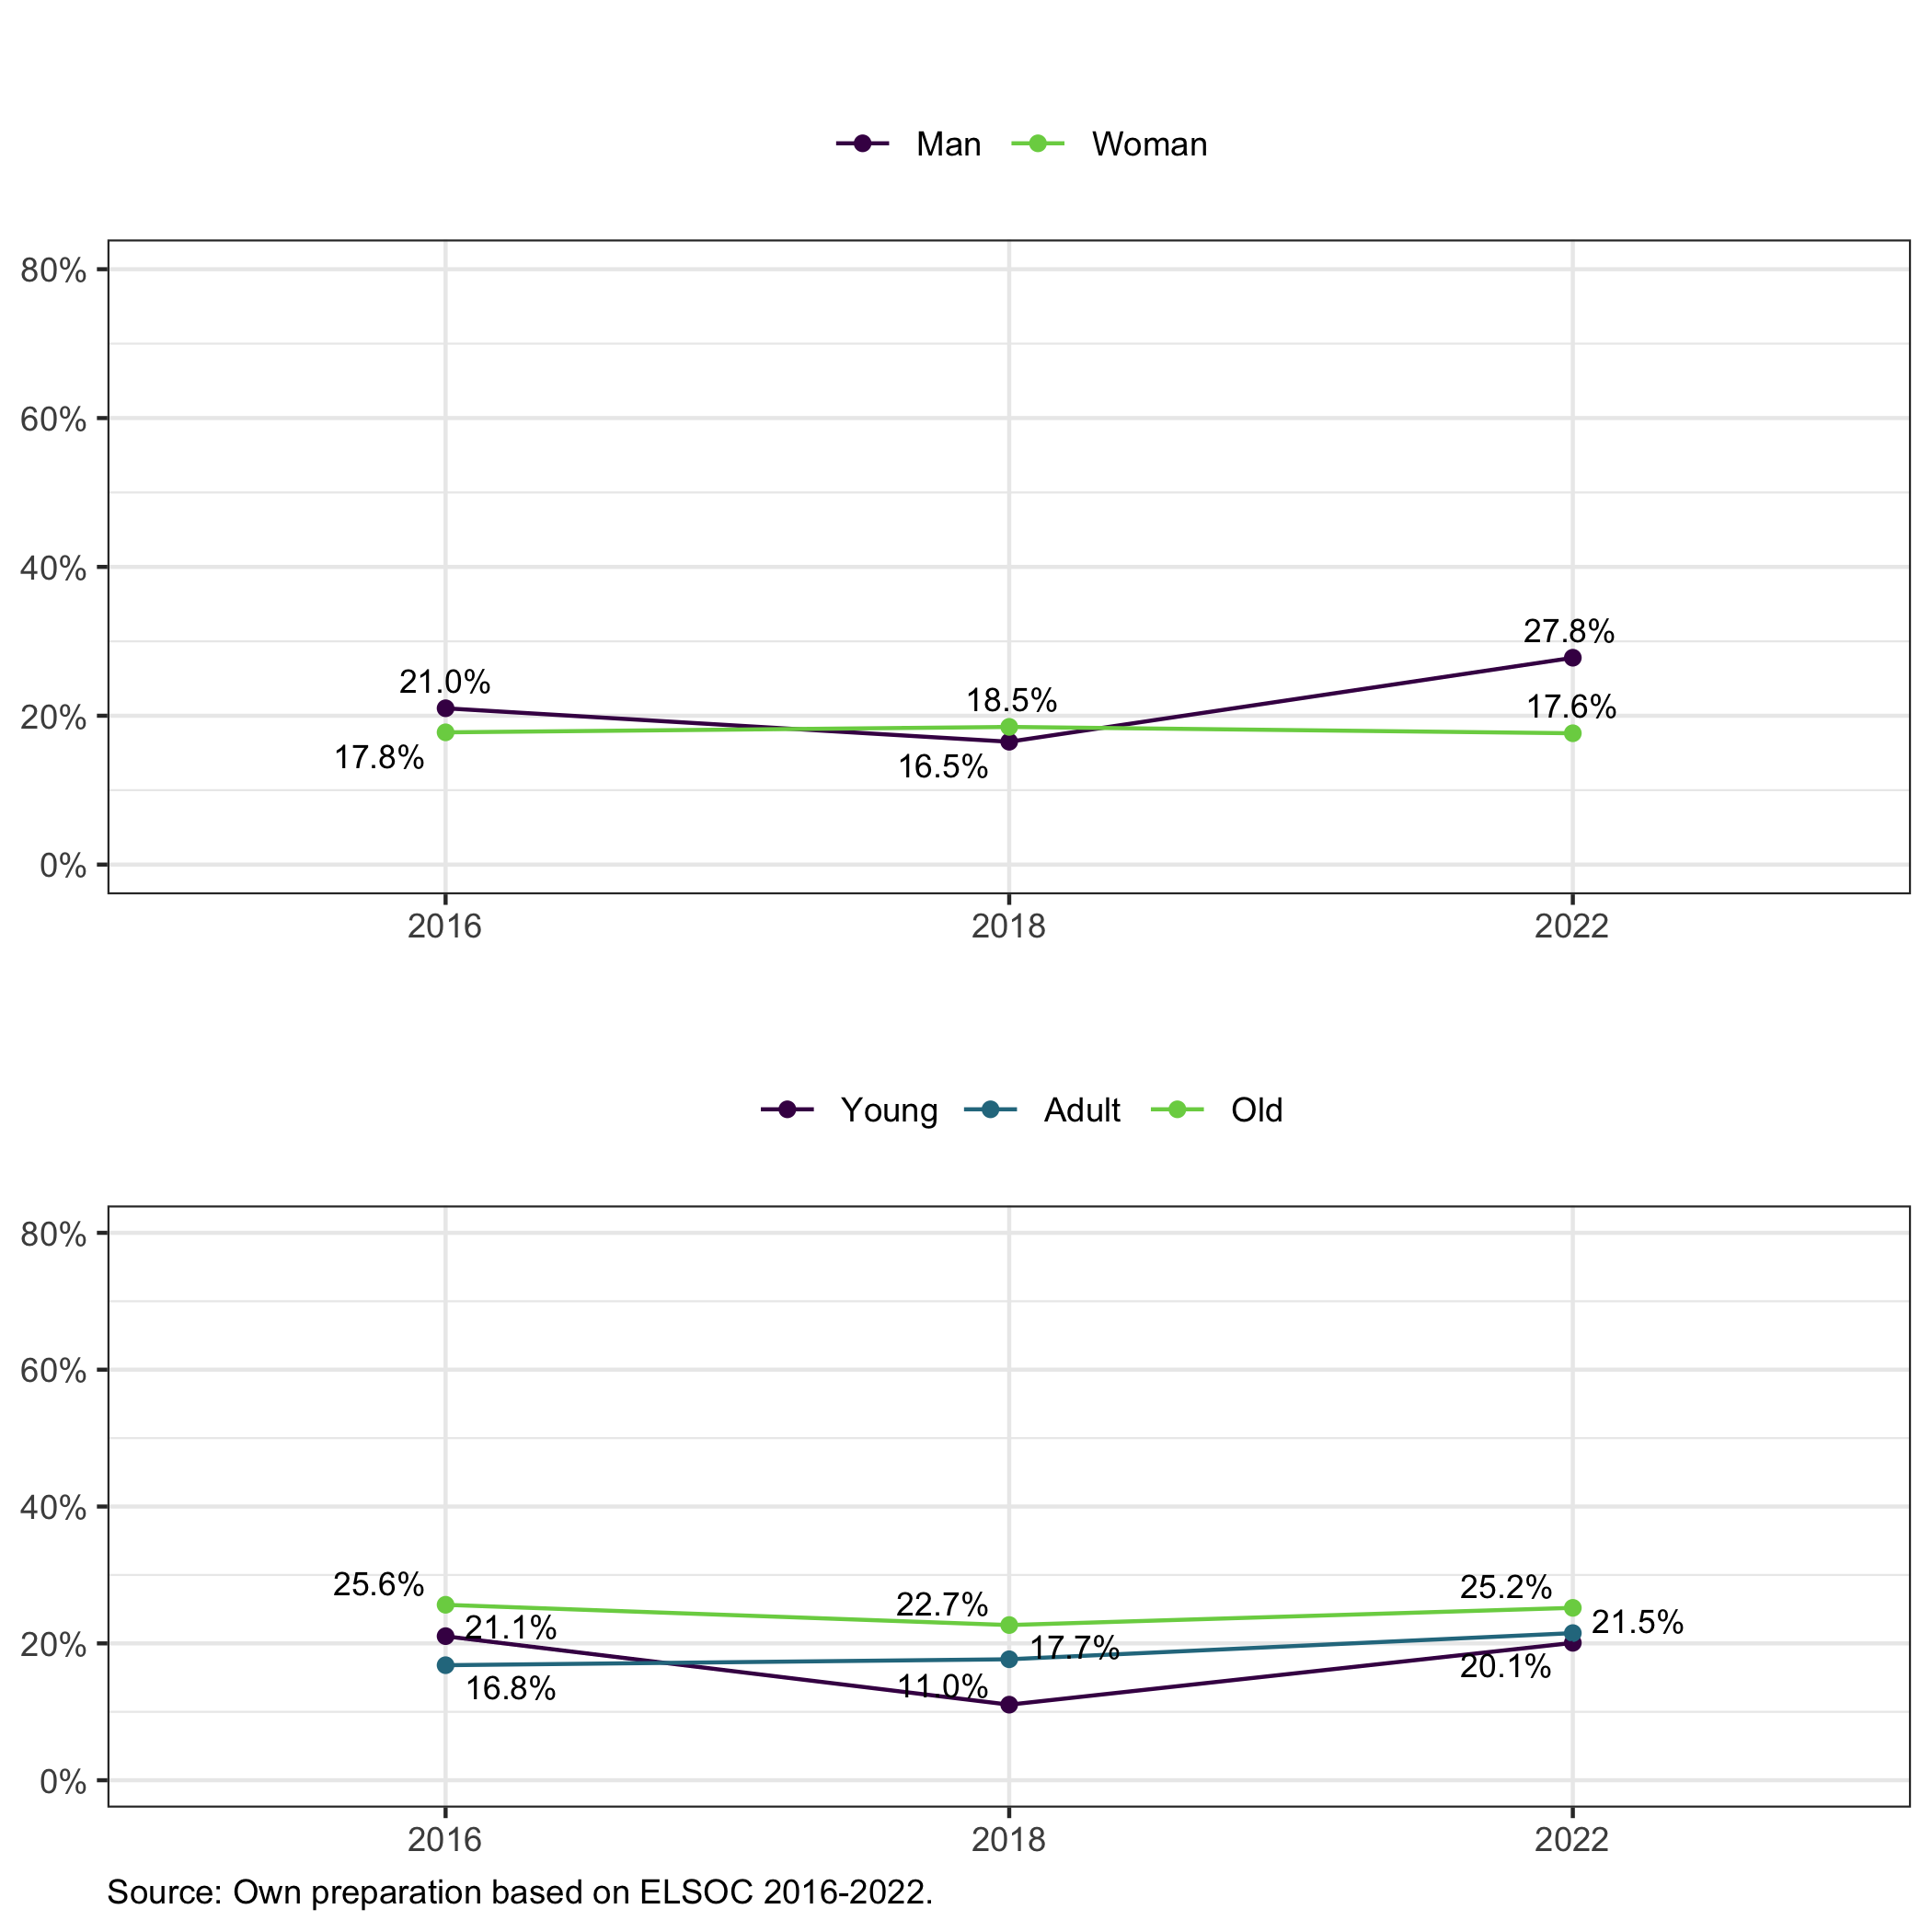
\includegraphics[width=16cm]{output/fig9.png}
    \caption{Active member of two or more organizations}
    \label{fig:fig9}
\end{figure}


\section{Results}


\begin{figure}[H]
    \centering
    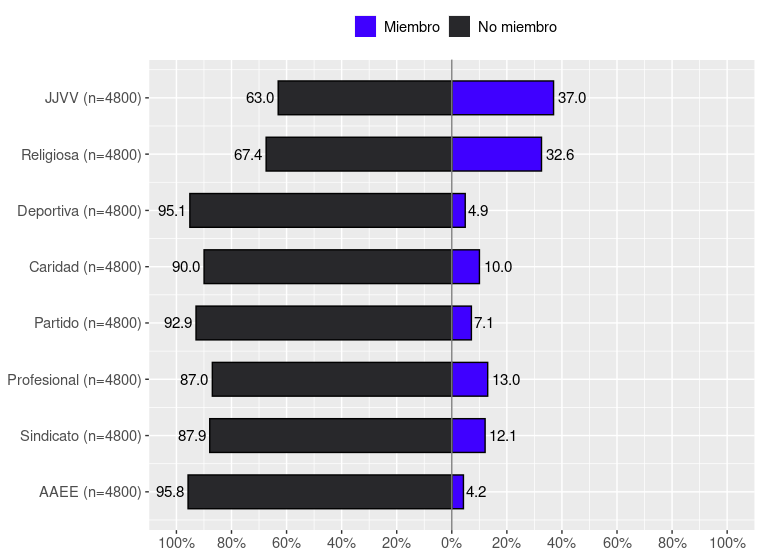
\includegraphics[width=13cm]{output/plot_items.png}
    \caption{Distribución de respuestas para las 3 olas del estudio}
    \label{fig:likert}
\end{figure}



\subsection{Latent class analysis}

Longitudinal classification models are based on a first-order homogeneous Markov chain with finite states. The maximum likelihood estimation of the model parameters is performed using the Expectation-Maximization (EM) algorithm, and the standard errors are obtained using parametric bootstrap. In addition, we include relevant covariates to describe the emergent groups or classes. This assumes that the response variables measure the individual characteristic of interest (the associative behavior) represented by the latent variables. This feature is not directly observable and may evolve. Indeed, our interest is to model the effect of the covariates on the latent distribution \parencite{bartolucci_latent_2009}. As Bartolucci \citeyear{bartolucci_latent_2015} suggests, a natural way to allow the initial and transition probabilities of the LM chain to depend on the individual covariates is through a logit multinomial parameterization:

\begin{equation}
log\frac{P(U^{1}=u|X^{(1)}=x)}{P(U^{1}=1|X^{(1)}=x)}=log\frac{\pi_{u}|x}{\pi_{1}|x}=\beta_{0u}+x^\top \beta_{1u}, u=2,...,k,
\end{equation}


\begin{equation}
log\frac{P(U^{(t)}=u|U^{(t-1)}=\overline{u},X^{(t)}=x)}{P(U^{(t)}=\overline{u}|U^{(t-1)}=\overline{u},X^{(t)}=x)} = log\frac{\pi^{(t)}_{u|\overline{u}x}}{\pi^{(t)}_{\overline{u}|\overline{u}x}}=\gamma_{0\overline{u}u}+x^{\top}\gamma_{1\overline{u}u},
\end{equation}

for \( t=2,...,T \) and \( \overline{u}, u = 1,...,k, \) with \( \overline{u} \neq u\). In the above expression, \( \beta_u = (\beta_{0u},\beta^\top_{1u})^\top\) and \(\gamma_{\overline{u}u}=(\gamma^\top_{1\overline{u}u})^\top \) are parameter vector to be estimated which are collected in the matrices \(\beta \) and \( \Gamma \). As already mentioned, when the covariates affect the distribution of the latent process, these covariates are typically excluded from the measurement model and we adopt the constraint \( \phi^{(t)}_{jy|ux}=\phi_{jy|u}\) \parencite{bartolucci_lmest_2017}. 





% latex table generated in R 4.1.2 by xtable 1.8-4 package
% Thu Jun  1 17:43:38 2023
\begin{table}[H]
\centering
\begin{threeparttable}
\caption{\label{demo-table} Fit statistics of class models}
\begin{tabular}{rrrrrr}
  \hline
 & states & lk & np & aic & bic \\ 
  \hline
1 & 1.00 & -14394.87 & 8.00 & 28805.74 & 28848.76 \\ 
  2 & 2.00 & -13586.64 & 46.00 & 27265.28 & 27512.66 \\ 
  3 & 3.00 & -12965.46 & 104.00 & 26138.91 & 26698.20 \\ 
  4 & 4.00 & -12734.50 & 102.00 & 25833.01 & 26811.76 \\ 
  5 & 5.00 & -12523.17 & 200.00 & 25606.33 & 27112.11 \\ 
   \hline
\end{tabular}
\begin{tablenotes}
    \item[1] According to the BIC relative fit statistic, the 3-class model has the best fit.
  \end{tablenotes}
\end{threeparttable}
\end{table}

The models are evaluated considering the BIC relative fit statistic. This statistic is generally preferred to the AIC statistic, and the model with the smaller number represents the best configuration of goodness-of-fit and complexity \parencite{bartolucci_latent_2015}. Based on Table 1, the model corresponding to the minimum BIC is that with k = 3 latent states. 

\begin{figure}[htp]
    \centering
    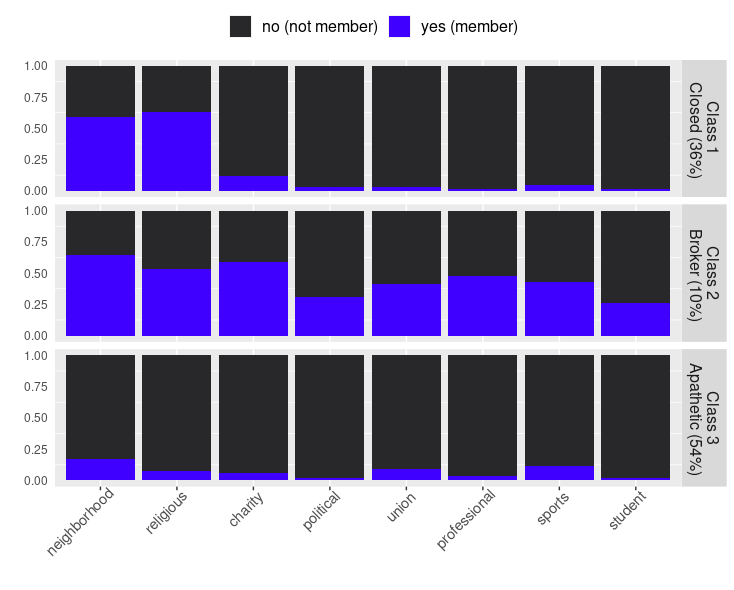
\includegraphics[width=13cm]{output/plot_latentclass2.png}
    \caption{Estimates conditional response probabilities}
    \label{fig:}
\end{figure}


Figure 2 illustrates the estimated conditional response probabilities \( \widehat{\phi}_{y|u}\). We can generally observe that the individuals in the first latent state, which we call "Closed," represent 36 \% of the samples. These individuals present an associative behavior centered on two voluntary associations: neighborhood and religious. A particular aspect of this type of association is that they have solid territorial roots and which limits their ability to influence the local sphere. For its part, the latent state or class two, which we call "brokers," comprises individuals with probabilities of over .35 memberships in all types of voluntary associations, highlighting the likelihood of being a member of charitable organizations, professionals, and unions. This group and its multiple memberships facilitate articulation, the flow of information, and contagion (e.g., cultural) between different types of associations. This can be considered a structural quality that gives an advantage to individuals while contributing to organizational development and connectivity of the civil society field. Finally, class or state 3 is the majority since it represents 54\% of the sample. We call this class of individuals "apathetic" since they present very low probabilities of participating in associative types. It is worth noting that this pattern of associative behavior has been analyzed and conceptualized as a tendency to withdraw to the private space.


% latex table generated in R 4.1.2 by xtable 1.8-4 package
% Thu Jun  1 19:02:37 2023
\begin{table}[H]
\centering
\begin{threeparttable}
\caption{\label{demo-table} Multinomial regression}
\begin{tabular}{rrr}
  \hline
 & Class 2 (broker) & Class 3 (apathetic)\\ 
  \hline
Intercept & -1.66** & 1.56*** \\ 
  Mujer & -1.46*** & -1.32*** \\ 
  25-34 & 0.24 & -0.16 \\ 
  35-44 & 0.46 & -0.53 \\ 
  45-54 & 0.47 & -0.70 \\ 
  55-64 & -0.15 & -1.19** \\ 
  65- & -0.67 & -1.72*** \\ 
  Media & 0.82* & 0.49* \\ 
  Técnica & 1.40** & 1.00** \\ 
  Universitaria & 3.24*** & 1.57*** \\ 
   \hline
\multicolumn{3}{l}{\textsuperscript{***}$p<0.01$, 
  \textsuperscript{**}$p<0.05$, 
  \textsuperscript{*}$p<0.1$}
\end{tabular}
\begin{tablenotes}
    \item[1] Class 1 (closed) is reference category.
  \end{tablenotes}
\end{threeparttable}
\end{table}

Table 3 contains the estimated regression parameters that affect the distribution of the initial probabilities obtained with Equation 5. The logarithmic possibilities of gender are all negative, indicating that initially (time 1), women are less likely to belong to the latent states "runner" and "listless." On the other hand, individuals in the "intermediate" class are more likely to have higher educational levels than the "closed" class. The same is true for the "apathetic" class. Specifically, for the "broker" class, the odds ratio of having a college education is 25 times higher, and for the "apathetic" class, it is 4.8 times higher, in contrast to the "closed" class.


\begin{figure}[htp]
    \centering
    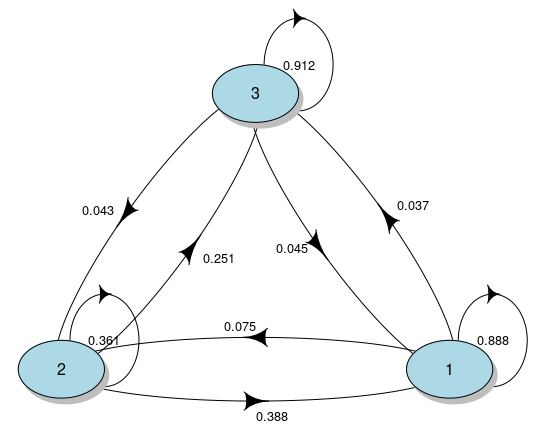
\includegraphics[width=11cm]{output/plot_transition.png}
    \caption{Averaged transition probabilities}
    \label{fig:galaxy}
\end{figure}


\section{Discussion}

\section{Conclusion}

- The low level of membership in voluntary associations in Chile is notable.
- The associative behavior pattern that we call “broker” is the least numerous and least stable over time.
- It is remarkable that the pattrn “broker” accumulates the largest number of people who trust other strangers
- At the same time, it is the pattern that accumulates the most diversity.
- Finally, it is noteworthy that the pattern that least trusts others is the
closed one (which corresponds to our hypothesis) and that the difference, in favor of the “broker” class, is the strongest in relation to the others.

\newpage

\printbibliography

\newpage

\section{Supplementary analysis}

\begin{table}[ht]
\centering
\caption{CFA generalized trust wave 1}
\label{tab:conf1}
\begin{tabular}{@{}r *{2}{S[table-format=2.2]}}
\toprule
& \multicolumn{2}{c}{Model} \\
\midrule
& Estimate & p \\
\midrule
\multicolumn{4}{c}{\underline{Factor Loadings}} \\
\multicolumn{1}{l}{\underline{Confianza}} \\
Confianza general & 0.72 & 0.000 \\
Altruismo general & 0.75 & 0.000 \\
La gente trata de ser justa & 0.66 & 0.000 \\
\midrule
\multicolumn{4}{c}{\underline{Fit Indices}} \\
$\chi^2(\text{df})$ & 0.00 &  \\
RMSEA & 0.00 &  \\
Scaled $\chi^2(\text{df})$ & 0.00(0) &  \\
\bottomrule
\end{tabular}
\end{table}


\begin{table}[ht]
\centering
\caption{CFA generalized trust wave 3}
\label{tab:conf2}
\begin{tabular}{@{}r *{2}{S[table-format=2.2]}}
\toprule
& \multicolumn{2}{c}{Model} \\
\midrule
& Estimate & p \\
\midrule
\multicolumn{4}{c}{\underline{Factor Loadings}} \\
\multicolumn{1}{l}{\underline{CONF}} \\
Confianza general & 0.72 & 0.000 \\
Altruismo general & 0.75 & 0.000 \\
La gente trata de ser justa & 0.63 & 0.000 \\
\midrule
\multicolumn{4}{c}{\underline{Fit Indices}} \\
$\chi^2(\text{df})$ & 0.00 &  \\
RMSEA & 0.00 &  \\
Scaled $\chi^2(\text{df})$ & 0.00(0) &  \\
\bottomrule
\end{tabular}
\end{table}


\begin{table}[ht]
\centering
\caption{CFA generalized trust wave 6}
\label{tab:conf}
\begin{tabular}{@{}r *{2}{S[table-format=2.2]}}
\toprule
& \multicolumn{2}{c}{Model} \\
\midrule
& Estimate & p \\
\midrule
\multicolumn{4}{c}{\underline{Factor Loadings}} \\
\multicolumn{1}{l}{\underline{Confianza}} \\
Confianza general & 0.61 & 0.000 \\
Altruismo general & 0.63 & 0.000 \\
La gente trata de ser justa & 0.74 & 0.000 \\
\midrule
\multicolumn{4}{c}{\underline{Fit Indices}} \\
$\chi^2(\text{df})$ & 0.00 &  \\
RMSEA & 0.00 &  \\
Scaled $\chi^2(\text{df})$ & 0.00(0) &  \\
\bottomrule
\end{tabular}
\end{table}
 


\end{document}
